\documentclass[tikz,border=12pt]{standalone}
\usepackage[T1]{fontenc}
\usepackage{tgheros}
\usepackage{sfmath}
\usepackage{amsmath,amssymb}
% % \usepackage{fontawesome5} (Removed for publication-grade academic typography) (Removed for publication-grade academic typography)
\usepackage{tikz}
\usetikzlibrary{arrows.meta,positioning,shapes.geometric,fit,backgrounds,calc}
\usepackage{xcolor}

\renewcommand{\familydefault}{\sfdefault}

% Canonical Semantic Palette
\definecolor{structuralnavy}{HTML}{1B2A4A}
\definecolor{measuredteal}{HTML}{168F84}
\definecolor{proposalamber}{HTML}{C98218}
\definecolor{consequencecoral}{HTML}{BD4F2F}
\definecolor{authorityviolet}{HTML}{6550A8}
\definecolor{neutralgray}{HTML}{687386}
\definecolor{navyfill}{HTML}{E8EDF6}
\definecolor{tealfill}{HTML}{E4F6F3}
\definecolor{amberfill}{HTML}{FFF3DC}
\definecolor{coralfill}{HTML}{FAE9E2}
\definecolor{grayfill}{HTML}{F4F6F7}
\definecolor{cardborder}{HTML}{CBD5E1}

\begin{document}
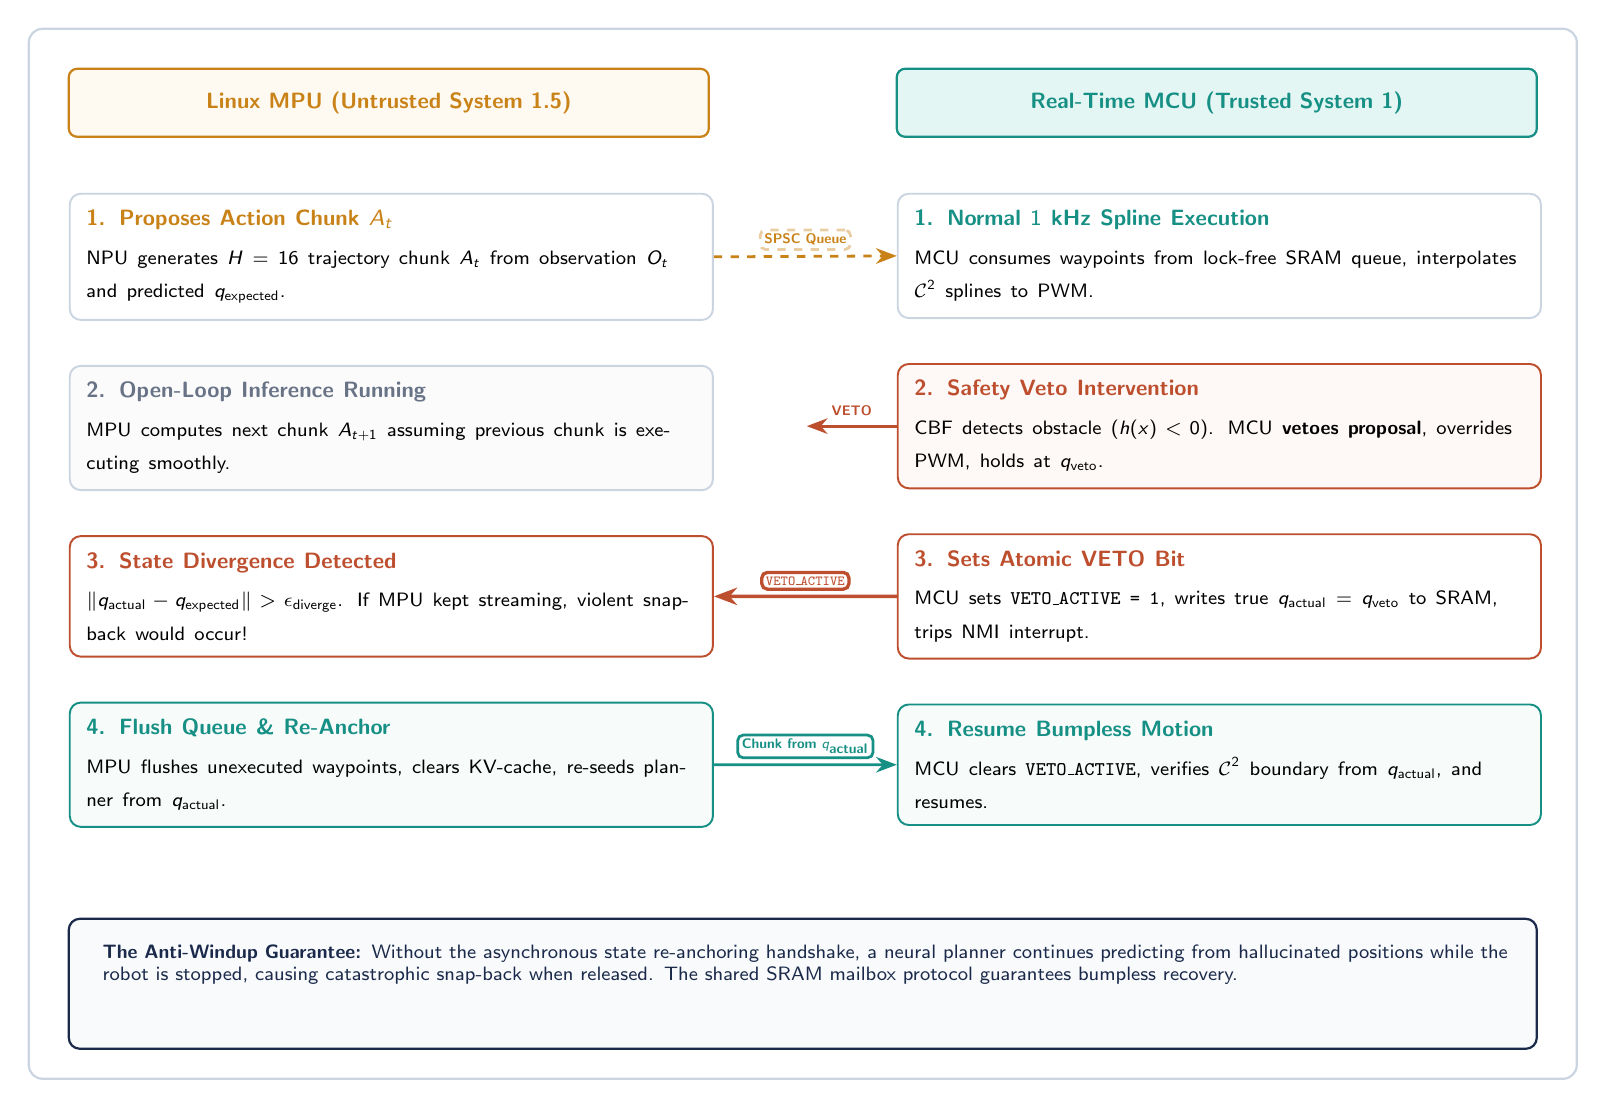
\begin{tikzpicture}[
  font=\sffamily,
  >=Stealth,
  card/.style={
    draw=cardborder,
    fill=white,
    rounded corners=5pt,
    line width=0.8pt,
    inner sep=8pt
  },
  stepcard/.style={
    draw=cardborder,
    fill=white,
    rounded corners=4pt,
    line width=0.7pt,
    inner sep=6pt,
    text width=3.05in,
    align=left
  }
]

  % Main Container Card
  \coordinate (c_top) at (0, 0);
  \draw[draw=cardborder, fill=white, rounded corners=5pt, line width=0.8pt] 
    (c_top) rectangle ++(7.74in, -5.25in);

  % ----------------------------------------------------
  % 2 ARCHITECTURAL COLUMNS (MPU vs MCU)
  % ----------------------------------------------------
  \coordinate (mpu_hdr) at ($(c_top) + (0.2in, -0.20in)$);
  \draw[draw=proposalamber, fill=amberfill!40, rounded corners=3pt, line width=0.8pt]
    (mpu_hdr) rectangle ++(3.20in, -0.34in);
  \node[font=\footnotesize\bfseries, color=proposalamber] at ($(mpu_hdr) + (1.60in, -0.17in)$) {
     Linux MPU (Untrusted System 1.5)
  };

  \coordinate (mcu_hdr) at ($(c_top) + (4.34in, -0.20in)$);
  \draw[draw=measuredteal, fill=tealfill, rounded corners=3pt, line width=0.8pt]
    (mcu_hdr) rectangle ++(3.20in, -0.34in);
  \node[font=\footnotesize\bfseries, color=measuredteal] at ($(mcu_hdr) + (1.60in, -0.17in)$) {
     Real-Time MCU (Trusted System 1)
  };

  % ----------------------------------------------------
  % PHASE 1: Normal Chunk Proposal
  % ----------------------------------------------------
  \node[stepcard, draw=cardborder, below=0.62in of mpu_hdr.south west, anchor=north west] (p1mpu) {
    \textbf{\footnotesize\color{proposalamber}1. Proposes Action Chunk $A_t$}\\[2pt]
    {\scriptsize NPU generates $H=16$ trajectory chunk $A_t$ from observation $O_t$ and predicted $q_{\text{expected}}$.}
  };

  \node[stepcard, draw=cardborder, below=0.62in of mcu_hdr.south west, anchor=north west] (p1mcu) {
    \textbf{\footnotesize\color{measuredteal}1. Normal $1\text{ kHz}$ Spline Execution}\\[2pt]
    {\scriptsize MCU consumes waypoints from lock-free SRAM queue, interpolates $\mathcal{C}^2$ splines to PWM.}
  };

  % Arrow P1: MPU -> MCU
  \draw[->, line width=1.0pt, proposalamber, dashed] (p1mpu.east) -- (p1mcu.west)
    node[midway, above=2pt, font=\tiny\bfseries, fill=white, draw=proposalamber!40, rounded corners=2pt, inner sep=1.5pt] {SPSC Queue};

  % ----------------------------------------------------
  % PHASE 2: Safety Veto & Intervention
  % ----------------------------------------------------
  \node[stepcard, draw=cardborder, fill=grayfill!40, below=0.22in of p1mpu.south west, anchor=north west] (p2mpu) {
    \textbf{\footnotesize\color{neutralgray}2. Open-Loop Inference Running}\\[2pt]
    {\scriptsize MPU computes next chunk $A_{t+1}$ assuming previous chunk is executing smoothly.}
  };

  \node[stepcard, draw=consequencecoral, fill=coralfill!30, below=0.22in of p1mcu.south west, anchor=north west] (p2mcu) {
    \textbf{\footnotesize\color{consequencecoral}2. Safety Veto Intervention}\\[2pt]
    {\scriptsize CBF detects obstacle ($h(x) < 0$). MCU \textbf{vetoes proposal}, overrides PWM, holds at $q_{\text{veto}}$.}
  };

  % Divergence indicator
  \draw[->, line width=1.0pt, consequencecoral] (p2mcu.west) -- ++(-0.45in, 0)
    node[midway, above, font=\tiny\bfseries] { VETO};

  % ----------------------------------------------------
  % PHASE 3: SRAM Mailbox Flag & State Divergence
  % ----------------------------------------------------
  \node[stepcard, draw=consequencecoral, fill=white, below=0.22in of p2mpu.south west, anchor=north west] (p3mpu) {
    \textbf{\footnotesize\color{consequencecoral}3. State Divergence Detected}\\[2pt]
    {\scriptsize $\|q_{\text{actual}} - q_{\text{expected}}\| > \epsilon_{\text{diverge}}$. If MPU kept streaming, violent snap-back would occur!}
  };

  \node[stepcard, draw=consequencecoral, fill=white, below=0.22in of p2mcu.south west, anchor=north west] (p3mcu) {
    \textbf{\footnotesize\color{consequencecoral}3. Sets Atomic VETO Bit}\\[2pt]
    {\scriptsize MCU sets \texttt{VETO\_ACTIVE = 1}, writes true $q_{\text{actual}} = q_{\text{veto}}$ to SRAM, trips NMI interrupt.}
  };

  % Arrow P3: MCU -> MPU Mailbox Flag
  \draw[->, line width=1.2pt, consequencecoral] (p3mcu.west) -- (p3mpu.east)
    node[midway, above=2pt, font=\tiny\bfseries, fill=white, draw=consequencecoral, rounded corners=2pt, inner sep=1.5pt] { \texttt{VETO\_ACTIVE}};

  % ----------------------------------------------------
  % PHASE 4: Pipeline Flush & Bumpless Re-Anchoring
  % ----------------------------------------------------
  \node[stepcard, draw=measuredteal, fill=tealfill!30, below=0.22in of p3mpu.south west, anchor=north west] (p4mpu) {
    \textbf{\footnotesize\color{measuredteal}4. Flush Queue \& Re-Anchor}\\[2pt]
    {\scriptsize MPU flushes unexecuted waypoints, clears KV-cache, re-seeds planner from $q_{\text{actual}}$.}
  };

  \node[stepcard, draw=measuredteal, fill=tealfill!30, below=0.22in of p3mcu.south west, anchor=north west] (p4mcu) {
    \textbf{\footnotesize\color{measuredteal}4. Resume Bumpless Motion}\\[2pt]
    {\scriptsize MCU clears \texttt{VETO\_ACTIVE}, verifies $\mathcal{C}^2$ boundary from $q_{\text{actual}}$, and resumes.}
  };

  % Arrow P4: Resumption
  \draw[->, line width=1.0pt, measuredteal] (p4mpu.east) -- (p4mcu.west)
    node[midway, above=2pt, font=\tiny\bfseries, fill=white, draw=measuredteal, rounded corners=2pt, inner sep=1.5pt] {Chunk from $q_{\text{actual}}$};

  % ----------------------------------------------------
  % BOTTOM TAKEAWAY BANNER
  % ----------------------------------------------------
  \coordinate (bot_pos) at ($(c_top) + (0.2in, -4.45in)$);
  \draw[draw=structuralnavy, fill=navyfill!30, rounded corners=4pt, line width=0.8pt]
    (bot_pos) rectangle ++(7.34in, -0.65in);

  \node[anchor=north west, font=\scriptsize, text width=7.15in, align=left, color=structuralnavy] at ($(bot_pos) + (0.12in, -0.08in)$) {
    \textbf{\color{structuralnavy} The Anti-Windup Guarantee:} Without the asynchronous state re-anchoring handshake, a neural planner continues predicting from hallucinated positions while the robot is stopped, causing catastrophic snap-back when released. The shared SRAM mailbox protocol guarantees bumpless recovery.
  };

\end{tikzpicture}
\end{document}
